\documentclass{ieeeaccess}
\usepackage{cite}
\usepackage{amsmath,amssymb,amsfonts}
\usepackage{algorithm}
\usepackage{algorithmicx}
\usepackage{algpseudocode}
%% \usepackage{caption}
\usepackage{graphicx}
\usepackage{textcomp}
\def\BibTeX{{\rm B\kern-.05em{\sc i\kern-.025em b}\kern-.08em
    T\kern-.1667em\lower.7ex\hbox{E}\kern-.125emX}}
\begin{document}
\history{Date of publication xxxx 00, 0000, date of current version xxxx 00, 0000.}
\doi{10.1109/ACCESS.2017.DOI}

\title{Using Intuitionistic Fuzzy Inference Systems For the Creation
of an Agent-based Financial Market Model}
\author{
  \uppercase{Amaury Hernandez-Aguila\authorrefmark{1}
    and
    \uppercase{Mario Garcia-Valdez\authorrefmark{2}}}}
%% TODO: Check correct address. Can we use a single authorrefmark for
%% both authors?
\address[1]{National Institute of Standards and 
Technology, Boulder, CO 80305 USA (e-mail: author@boulder.nist.gov)}
\address[2]{Department of Physics, Colorado State University, Fort Collins, 
  CO 80523 USA (e-mail: author@lamar.colostate.edu)}
%% TODO: Grant information.
\tfootnote{This paragraph of the first footnote will contain support 
information, including sponsor and financial support acknowledgment. For 
example, ``This work was supported in part by the U.S. Department of 
Commerce under Grant BS123456.''}

%% TODO: What is this?
\markboth
{Author \headeretal: Preparation of Papers for IEEE TRANSACTIONS and JOURNALS}
{Author \headeretal: Preparation of Papers for IEEE TRANSACTIONS and JOURNALS}

\corresp{Corresponding author: Amaury Hernandez-Aguila (e-mail: amherag@tectijuana.edu.mx).}

\begin{abstract}
%% Highlights:
%% * The proposed method uses a multi-agent system for the creation of
%% financial market forecasting agent-based models.
%% * Intuitionistic fuzzy systems are used to model agents' knowledge.
%% * The resulting predictive models can be interpreted to obtain additional
%% insight about the financial markets they are modelling.
%% * The resulting predictive models are competent for the forecasting of
%% market prices.

Many methods for the creation of financial market models exist, such as linear
regression and neural networks. However, the models created by many of these
methods provide little to no additional insight regarding the problem they are
modelling---one can contrast the models generated by neural networks against
those generated by decision trees, as an example. The models generated by the
method proposed in this paper, in addition to the expected forecasting of
market prices, can be examined to provide possible explanations of how the
prices of a market are formed. The proposed method uses a multi-agent system
where agent rules are modelled using intuitionistic fuzzy systems. This
approach allows the compilation of model interpretations for financial markets
from both macro and micro perspectives, as one can draw inferences about how
both the interaction among the agents and each individual agent's knowledge
affect the prices of a market. In addition to its interpretation capabilities,
the proposed method demonstrates its efficacy for the creation of competent
predictive models.
\end{abstract}

\begin{keywords}
  %% TODO: Review keywords.
  %% I'm already using kewords from
  %% http://www.ieee.org/organizations/pubs/ani_prod/keywrd98.txt
decision support systems, economic forecasting, fuzzy systems,
multi-agent system
\end{keywords}

\titlepgskip=-15pt

\maketitle

\section{Introduction}
\label{section:introduction}

%% Amaury: Tweak introduction following highlights.

A financial market is constructed by the interactions of a number of traders,
where a trader is an entity that is able to buy or sell a number of units of an
asset. The traders can either be individual human beings, organizations or even
computer programs. An asset can be anything that can be priced and can be
divided so different parties can hold a share of the asset. For example, corn
can be priced and different parties can hold a share of the corn market by
physically owning corn. Lastly, traders can decide to either buy or sell shares
of this asset. Although this decision can seem simple, as there can only be two
outcomes, the process a trader can follow in order to arrive to an outcome can
be very complex.

In theory, if one can know all the variables that each trader is taking into
consideration to arrive to their particular decisions, the prices in a financial
market can be predicted precisely. Obviously, this is near impossible, unless we
were simulating a financial market with a handful of people and everyone was
telling everyone else what decisions they are going to be taking. Nevertheless,
one can create models that closely simulate a financial market, and one can
assume that these simulations are generalizations of the real financial
market. Several approaches have been taken in the past to create such models
with varying success. One of the simplest methods to forecast the prices in a
financial market is linear % % Amaury: Maybe use a more recent example. It
%% doesn't matter if we change the technique.
regression~\cite{kutner2004applied}, where one is trying to find a function of
the form $f(x) = a + bx$ --- or simply a linear function --- that minimizes the
distance between the points in the line and the points that represent the
prices. Even though linear regression can provide valuable insight, such as
determining the general direction of a market in a determined period of time, it
is not suitable to be taken as a complete solution to forecasting.

A better approach to using mathematical formulas to forecast a financial market
is to use technical indicators such as the relative strength index or the
commodity selection index~\cite{Wilder1978}. These technical indicators are used
to perform a technique called technical analysis, where one tries to identify
what are going to be the future price movements of a market relying solely on
the historical prices of the market being analyzed. For example, if a market's
prices have been increasing relatively too much in a relatively short period of
time, according to technical analysis this market is now considered
\textit{overbought}, and the prices could start to violently fall at any
moment. It is worth noting that these analyses are often subject to
interpretation, i.e.\ they are subjective analyses. Additionally, these analyses
are heuristic, as the trader's experience is heavily involved in the
interpretation of the results obtained by the technical indicators.

One method that does not need interpretation, unlike technical analysis, and
that creates a model that tries to simulate a financial market, like linear
regression, is artificial neural networks (ANN). ANN-based models are created by
using a series of data points --- in the case of financial markets, these data
points are historical prices --- as a training set, which is used to adjust
weights in the neurons that constitute the ANN.\@ In the end, an ANN is just a
very complex mathematical formula that, given an input, one obtains an output,
which in the case of a financial market, that output is a price at a given
time. Although ANNs can generate models that successfully simulate financial
markets, interpreting the model is sometimes desired, as one can obtain insight
that can help to better understand a market's behavior, and ANNs fail to
accomplish this goal.

Agent-based models satisfy two criteria: they are interpretable, as one can
examine what are the rules and beliefs that conveyed an agent to a particular
decision; and they can simulate a financial market, which helps to provide a
model that is closely related to that market's behavior, unlike technical
indicators. %
% Amaury: re-think the "unlike technical indicators". Is this true?
Furthermore, the agents in an agent-based model can use the outputs from several
technical indicators as the environment that works as the input to their rules,
instead of using the raw historical prices, which already implies that
agent-based models can act in a higher order of complexity than technical
indicators. For example, the historical prices of a financial market can be
pre-processed using technical indicators, and these will serve as the basis for
the agents' beliefs, such as believing if a market is overbought or oversold, or
if the volatility is too high or too low.

The representation of an agents' beliefs and rules can be achieved through
traditional (Boolean) logic, for example: \textit{if relative strength index is
greater than 20, then buy}. Nevertheless, fuzzy logic can help to achieve a
greater level of detail for the creation of the agents' rules and beliefs. The
aforementioned example rule can then be extended to \textit{if relative strength
index is low, then buy a big lot}. As can be noted, just as one can use fuzzy
logic to create fuzzy inference systems, the agents' actions can also be
represented by fuzzy rules.

The preceding paragraphs serve as a description of the motivation behind the
proposed method in this work: using fuzzy inference systems for the creation of
agent-based models. However, the reader will find in Section~\ref{section:proposed-method} that the proposed method does not use traditional
fuzzy systems, but intuitionistic fuzzy systems~\cite{Atanassov1986}, which have
the objective of better representing the knowledge and decisions of a human
trader. Before better examining the method for constructing such agent-based
models, a series of related works is presented in Section
\ref{section:state-of-the-art}, which helps the reader to understand the advantages
that the proposed method in this work provides in contrast to other already
existing techniques. After understanding the theoretical background of the
method, the reader can find an implementation of the method in Section
\ref{section:implementation}.
%
% Amaury: Explain structure of the paper.

\section{Preliminaries}
\label{section:preliminaries}
%
% Amaury: Maybe reduce the length of this section.

This Section describes the concepts that the reader needs to be familiar with in
order to better understand the proposed method in Section
\ref{section:proposed-method}.% If the reader is already familiarized with any
%% of the concepts discussed below, it can be omitted.
% Amaury: I don't know if it sounds weird to say it can be omitted.

\subsection{Fuzzy Sets}
\label{subsection:fuzzy-sets}

A traditional set is a collection of items that share a common
characteristic. This characteristic serves as a membership, because all the
items in a universe either have that characteristic --- and then the item is
part of the set --- or it does not have it --- and then the item is not part of
the set. Traditional sets can be extended to fuzzy sets, as explained by
Zadeh~\cite{Zadeh1965}.
Fuzzy sets are then a generalization of traditional sets,
i.e.\ any traditional set can be represented as a fuzzy set. The difference
between these two type of sets lies in the concept of membership: memberships
are not only used to represent binary outcomes, i.e. \textit{true} or
\textit{false}, but now a possibly infinite number of outcomes. An item can now
be partially a member of a set, and the only way an item is not part of such set
is if its membership is totally \textit{false}. In order to represent this grade
of membership one can use real numbers. Thus, one can say, for example, that an
item is \textit{0.7 green}, \textit{0.5 blue} and \textit{0.0 red}. These values
can represent an adverb and an adjective, such as ``very green,'' ``somewhat
blue'' and ``not red at all.'' This is especially useful when designing fuzzy
systems (see Subsection \ref{subsection:fuzzy-systems}).

\subsection{Fuzzy Systems}
\label{subsection:fuzzy-systems}

%% TODO: Linguistic hedges are often associated to these multiple membership
%% functions to describe them in a more comprehensible way.

In traditional logic one can generate logical inferences, such as \textit{if
it's raining, then there are clouds in the sky}. In a similar fashion, one can
use fuzzy sets to represent the antecedents and consequents in a logical
inference process. For example, one can extend the previous example to:
\textit{if it's raining a lot, then there are many clouds in the sky}.

There is a number of ways in which one can construct a fuzzy inference system,
where one or more inputs or antecedents can be used to generate one or more
outputs or consequents. Arguably, the two most popular types of fuzzy inference
systems are the ones created by Mamdani and Assilian~\cite{Mamdani1975}, and
Takagi and Sugeno~\cite{Takagi1985}. These systems use a series of fuzzy sets to
represent the relationship between an input and its grade of membership to a
set. These sets usually represent adjectives that describe the inputs, and are
also considered to be the antecedents in the fuzzy inference system. For
example, an input of 0.8 can represent a ``very high'' value. After obtaining
these grades of membership, one can use these values to ``fire'' or ``activate''
the consequents. In the case of a Mamdani system, the consequents are
represented as fuzzy sets, just like the antecedents. In contrast, in a Sugeno
system, consequents are represented by mathematical functions. A set of rules is
used to determine the relationship between the antecedents and the consequents,
for example: \textit{if food quality is high then tip is high}. The
aforementioned rule is creating a relationship between the fuzzy set that
represents ``high food quality'' in the antecedents, and the fuzzy set that
represents ``high tip'' in the consequents. Further continuing with the example,
if ``food quality'' is represented by a value of 0.8, the rule that creates the
relationship between ``food quality'' and ``tip'' could determine a ``tip'' of
0.8 too, depending on what membership function and what parameters are decided
to be used to represent each.

It has been explained how a relationship between antecedents and consequents can
be constructed in a fuzzy inference system. Nevertheless, the most interesting
problem arises when a problem involves several fuzzy sets to represent different
adjectives for single antecedents or consequents. In these cases, depending on
the fuzzy rules, a number of consequents can be fired according to the inputs to
the system. As seen in Figure \ref{figure:antecedents}, the input ---
represented by the dotted vertical black line --- is associated with three fuzzy
triangular sets or antecedents, where it ``activates'' two of them. According to
a set of fuzzy rules, it then fires a set of triangular fuzzy sets that
represent the consequents, as seen in Figure \ref{figure:consequents}.

The fuzzy sets that represent the consequents are cut, and new shapes are
obtained using those cuts, as represented by the green shapes in Figure
\ref{figure:consequents}. These shapes are aggregated and result in the output
of the fuzzy inference system, and this result can then be defuzzified using
different methods, such as obtaining the centroid of the shape. In this example,
a Mamdani fuzzy inference system is considered; in the case of a Sugeno system,
for example, the antecedents would be represented by arbitrary mathematical
functions, instead of membership functions representing shapes such as the
triangles in the example presented above.

\Figure[](topskip=0pt, botskip=0pt, midskip=0pt)
[width=0.6\linewidth]
{img/antecedents.png}
{Example of antecedents in a Mamdani fuzzy system.
  \label{figure:antecedents}}

\Figure[](topskip=0pt, botskip=0pt, midskip=0pt)
[width=0.6\linewidth]
{img/consequents.png}
{Example of consequents in a Mamdani fuzzy system.
  \label{figure:consequents}}

\subsection{Intuitionistic Fuzzy Sets}
\label{subsection:intuitionistic-fuzzy-sets}

In contrast to the traditional fuzzy sets discussed in Subsection
\ref{subsection:fuzzy-sets}, intuitionistic fuzzy sets consider a grade of
non-membership in addition to a grade of membership associated to an element in
the fuzzy set, as expressed by \ref{eq:ifs-definition}.

% intuitionistic fuzzy set
\begin{equation}
  \label{eq:ifs-definition}
  A^{*} = \{\langle x, \mu _{A} (x), \nu _{A} (x) \rangle | x \in E\}
\end{equation}

For every of the elements contained in an intuitionistic fuzzy set,
\ref{eq:intuitionistic-interval} must hold true.

% intuitionistic interval
\begin{equation}
  \label{eq:intuitionistic-interval}
  0 \leq \mu_{A}(x) + \nu_{A}(x) \leq 1
\end{equation}

Intuitionistic fuzzy sets are an extension to traditional fuzzy sets, as any
traditional fuzzy set can be expressed as a particular case of an intuitionistic
fuzzy set, as in \ref{eq:ifs-form}.

% every ordinary fuzzy set has the form
\begin{equation}
  \label{eq:ifs-form}
  \{ \langle x, \mu_{A}(x), 1 - \mu_{A}(x) \rangle | x \in E \}
\end{equation}

If the sum of the membership $\mu_{A}(x)$ and non-membership $\nu_{A}(x)$ of an
element is less than $1$, the concept of indeterminacy or hesitancy arises,
which is described by \ref{eq:indeterminacy}. Indeterminacy is used to represent
doubt in the grade of membership of an element in an intuitionistic fuzzy set
and is described by \ref{eq:indeterminacy}.

% if
\begin{equation}
  \label{eq:indeterminacy}
  \pi_{A}(x) = 1 - \mu_{A}(x) - \nu_{A}(x)
\end{equation}

Traditional fuzzy sets can be extended to increase their capabilities of
representing uncertainty by introducing the concept of footprint of
uncertainty. A footprint of uncertainty is achieved by extending the membership
function, where each of its values are now fuzzy sets themselves, instead of
crisp values. Indeterminacy serves a different purpose than the one of footprint
of uncertainty. Instead of extending the uncertainty provided by traditional
fuzzy sets, indeterminacy helps to model doubt. For example, if traditional
fuzzy sets can model the following sentence: ``the object is very hot'',
indeterminacy can model ``it is unsure that the object is very hot''.

\Figure[](topskip=0pt, botskip=0pt, midskip=0pt)
[width=0.6\linewidth]
{img/fs-as-ifs.pdf}
{Traditional fuzzy set represented as an intuitionistic fuzzy set.
  \label{figure:fs-as-ifs}}

\Figure[](topskip=0pt, botskip=0pt, midskip=0pt)
[width=0.6\linewidth]
{img/ifs-diff-mu-sd.pdf}
{Intuitionistic fuzzy set with membership and non-membership functions with different means and standard deviations.
  \label{figure:ifs-diff-mu-sd}}

\subsection{Intuitionistic Fuzzy Systems}
\label{subsection:intuitionistic-fuzzy-systems}

Intuitionistic fuzzy sets, like traditional fuzzy sets, can be used to create
inference systems. Antecedents and consequents in the system can be handled by
intuitionistic fuzzy sets, as in a Mamdani system~\cite{Mamdani1975}, or only
the antecedents and use mathematical functions for the consequents as in a
Sugeno system~\cite{Takagi1985}.

Different approaches have been taken in the past by different authors on how to
build intuitionistic fuzzy systems. The authors of the present paper have worked
in a particular way of achieving this type of systems, and the method is
described in~\cite{Hernandez-Aguila2016} and~\cite{Hernandez-Aguila2017-2}. The
method described in the aforementioned works is presented in this Subsection for
the reader as a reference implementation.

% handle inputs
% alpha-cuts
% defuzzification

As is explained in~\cite{Hernandez-Aguila2016}, in an IFIS, in order for an
antecedent to fire a consequent according to a set of fuzzy rules, the final
grade of membership of an element has to be expressed in terms of its grade of
membership and its grade of non-membership. The resulting grade of membership of
an element of $A$ is represented by $i\mu_{A}(x)$, and is defined in
(\ref{imembership}).

% i-membership
\begin{equation}
  \label{imembership}
  i\mu_{A}(x) = (\nu_{A}(x) + \mu_{A}(x))\mu_{A}(x)
\end{equation}

To perform an alpha-cut in a consequent, one has to separate it in two stages:
1) perform a traditional alpha-cut in the membership function following equation
(\ref{alpha-cut}), and then 2) perform an alpha-cut in the non-membership
function following equation (\ref{nmf-alpha-cut}).

\begin{equation}
  \label{alpha-cut}
  \alpha(\mu (x),\mu_{\alpha}) =
  \begin{cases}
    \mu (x), & \text{if}\ \mu (x) \leq \mu_{alpha}  \\
    \mu_{\alpha}, & \text{otherwise}
  \end{cases}
\end{equation}

\begin{equation}
  \label{nmf-alpha-cut}
  \alpha_{NMF}(\nu (x),\mu_{\alpha}) =
  \begin{cases}
    \nu (x), & \text{if}\ \nu (x) \geq \nu (\mu_{alpha})  \\
    \nu (\mu_{alpha}), & \text{otherwise}
  \end{cases}
\end{equation}

The aggregation of the fired consequents is performed by applying
(\ref{union-operator}) on the alpha-cuts.

\begin{equation}
  \label{union-operator}
  \begin{aligned}
    A \cup B  = &\{ \langle x, max(\mu_{A} (x), \mu_{B} (x)),\\
    &\quad min(\nu_{A} (x), \nu_{B} (x)) \rangle | x \in E \}
\end{aligned}
\end{equation}

The final modification to the traditional inference process in a FIS is made to
the center of area procedure. The equation to calculate the center of area of a
traditional fuzzy set is (\ref{center-of-area}). In order to implement a center
of area for an intuitionistic fuzzy set, one has to incorporate the concept of
$i\mu(x)$, giving as a result (\ref{if-coa}), and its simplification form
(\ref{if-coa-simplified}).

% CoA
\begin{equation}
  \label{center-of-area}
  A_{CoA} = \dfrac{\sum_{i=1}^{N} \mu(x_{i})
    x_{i}}{\sum_{i=1}^{N} \mu(x_{i})}
\end{equation}

%iCoA
\begin{equation}
  \label{if-coa}
  A_{iCoA} = \dfrac{\sum_{i=1}^{N} (\mu(x_{i}) + \nu(x_{i})) \mu(x_{i})
    x_{i}}{\sum_{i=1}^{N} (\mu(x_{i}) + \nu(x_{i})) \mu(x_{i})}
\end{equation}

%iCoA contracted
\begin{equation}
  \label{if-coa-simplified}
  A_{iCoA} = \dfrac{\sum_{i=1}^{N} i\mu_{A}(x) x_{i}}{\sum_{i=1}^{N}
    i\mu_{A}(x)}
\end{equation}

\Figure[](topskip=0pt, botskip=0pt, midskip=0pt)
[width=0.6\linewidth]
{img/fis-surface.png}
{Output surface for the tipping problem using a traditional fuzzy system.
  \label{figure:tipping-output-surface}}

\Figure[](topskip=0pt, botskip=0pt, midskip=0pt)
[width=0.6\linewidth]
{img/ifis-surface.png}
{Output surface for the tipping problem using an intuitionistic fuzzy system.
  \label{figure:ifis-tipping-output-surface}}

\subsection{Multi-agent Systems and Agent-based Models}
\label{subsection:multi-agent-systems-and-agent-based-models}

A multi-agent system is software that solves a problem using agents. Agents can
be seen themselves as programs that interact with their environment, which may
include other agents. Agents in the proposed method in this paper follow the
structure suggested by Shoham in~\cite{Shoham1993}, where agents have
beliefs and rules. Beliefs are used by agents to arrive to an interpretation of
their environment, and rules are used to arrive to actions to be performed by
the agent towards their environment. The agents in the system are constantly
sensing their environment to determine what actions to take according to their
beliefs and rules. Multi-agent systems have the objective of solving a practical
problem, unlike agent-based models which are more focused to providing a
simulation of a problem.

As mentioned before, agents can also be used to create agent-based models. These
models are used to represent a problem so a human being can analyze it and infer
new knowledge from it, or it can be used to better understand a problem.

The proposed method in this paper is both a multi-agent system and an
agent-based model. It is a multi-agent system in the sense that it can be used
to create a trading strategy, and it is an agent-based model because the agents
in the system can be analyzed to understand the state of the market that is
serving as the system's environment.

\section{State of the Art}
\label{section:state-of-the-art}

\subsection{Multi-Agent Systems}
\label{subsection:multi-agent-systems}

\subsubsection{Fuzzy Multi-Agent Systems}
\label{subsubsection:fuzzy-systems}

\subsection{Fuzzy Systems}
\label{subsection:fuzzy-systems}

\subsubsection{Intuitionistic Fuzzy Systems}
\label{subsubsection:intuitionistic-fuzzy-systems}

\subsection{Financial Forecasting}
\label{subsection:financial-forecasting}

\subsubsection{Fuzzy Systems}
\label{subsubsection:fuzzy-systems}

\subsubsection{Multi-Agent Systems}
\label{subsubsection:multi-agent-systems}

\section{Proposed Method}
\label{section:proposed-method}

The proposed method involves the use of a multi-agent system which acts in a
decentralized fashion. Whereas a centralized multi-agent system depends on an
agents which coordinate the actions and communication among the agents, a
decentralized multi-agent system involves the use of agents that act
autonomously~\cite{andreadis2014classification}. However, it can be noted that
the system proposed in this paper has a mechanism that averages the output of
the agents to their environment, and another mechanism which sends the input to
the agents. Although these mechanisms can be considered characteristic of
centralized multi-agent systems, they are not particularly complex processes
compared to the rest of the processes involved in the proposed method, which are
related to decentralized multi-agent systems.

The architecture followed by the multi-agent system is based on the one proposed
by Shoham~\cite{Shoham1993}. Particularly, the method presented in this paper
adopts the idea of designing agents as a set of beliefs and rules that dictate
how agents perceive and interact with their environment.

The following Subsections describe the proposed method in
detail. Subsection~\ref{subsection:agent-architecture} describes the structure
followed by each of the agents that shape a predictive model, while
Subsection~\ref{subsection:multi-agent-system} describes how the agents in the
predictive model are coordinated and how they interact with their
environment. Finally, Subsection~\ref{subsection:meta-heuristic} describes a
meta-heuristic that finds a combination of agents that is suitable to be used
as a predictive model for particular data sets.

\subsection{Agent Architecture}
\label{subsection:agent-architecture}

Agent rules are defined by Mamdani intuitionistic fuzzy inference systems. Fuzzy systems
are convenient, as they can be interpreted, as opposed to, for example, neural
networks, where the weights associated to the neurons and the connections among
themselves become obscure to interpretation. Furthermore, the use of
intuitionistic fuzzy systems provides an additional layer for interpretation:
indeterminacy.

Indeterminacy surges as a consequent of the inclusion of non-membership to a
fuzzy system (see Subsection~\ref{subsection:intuitionistic-fuzzy-sets}). This
concept allows the designer of a fuzzy system to model doubt or hesitancy in a
data set. In the proposed method, indeterminacy is obtained in a heuristical
manner, as part of the optimization algorithm that searches for a combination of
agents that are used to create a predictive model.

The membership functions in the fuzzy systems are always defined as Gaussian
functions, although in future experiments this design choice can
change. Gaussian membership functions were chosen because of their capability of
modelling knowledge in a smoother way than their alternatives, such as
triangular or trapezoidal membership functions. Although other membership
functions can be better suited for certain situations, the proposed method is
currently designed for the creation of predictive models for arbitrary data sets,
where solutions are found using a meta-heuristic.

%% It is usual for a fuzzy rule to contain multiple membership functions to
%% describe input and output variables.

%% Amaury: Mention inputs and outputs in training data set.

In the proposed method, at least two Gaussian membership functions are used to
describe each agent rule antecedents and consequents. The mean of each Gaussian
membership function is equal to a random data point from the training data set,
while the spread of the Guassian membership functions that represent a fuzzy
rule will be equal to the standard deviation of the aforementioned randomly
chosen data points. In the case of the antecedents, the means are equal to data
points from the training data set that represent inputs, while outputs in the
training data set are used as the means for the membership functions that form
the consequents. This is expressed by
\ref{equation:membership-function-spread} and depicted in
Figure~\ref{figure:fuzzy-system-architecture}.

% TODO: Express standard deviation of randomly chosen data points.
\begin{equation}
  \label{equation:membership-function-spread}
  A_{iCoA} = \dfrac{\sum_{i=1}^{N} i\mu_{A}(x) x_{i}}{\sum_{i=1}^{N}
    i\mu_{A}(x)}
\end{equation}

\Figure[](topskip=0pt, botskip=0pt, midskip=0pt)
[width=0.6\linewidth]
{img/antecedents.png}
{Depiction of the fuzzy system architecture.
  \label{figure:fuzzy-system-architecture}}

Data points are used as the means of the membership functions as this guarantees
an agent to be able to react to at least those input values. On the other hand,
using the standard deviation of those chosen data points as the spread of the
Gaussian membership functions guarantees that uncertainties associated to each
membership function will affect ---in terms of fuzzy inferences--- at least one of
the other membership functions. If none of the membership functions were
affecting in any way the rest of the membership functions, the use of a fuzzy
system to represent the agent rules would be meaningless.

The domain of each membership function is not fixed as it is determined by the
chosen data points and their standard deviation. The calculation that determines
the domain of a membership function is expressed by~\ref{equation:mf-domain}, and---as a consequent of this
calculation---the domain of either the antecedents or the consequents in a fuzzy
system is expressed by~\ref{equation:ant-con-domain}. %% As can be seen in
%% the latter, the domain of both the antecedents and consequents is
%% determined by the minimum and the maximum values contained by the union of

%% Amaury: Talk about the range of the membership functions. As we're using
%% intuitionistic fuzzy sets, the core is not necessarily 1.0.

\begin{equation}
  \label{equation:mf-domain}
  A_{iCoA} = \dfrac{\sum_{i=1}^{N} i\mu_{A}(x) x_{i}}{\sum_{i=1}^{N}
    i\mu_{A}(x)}
\end{equation}

\begin{equation}
  \label{equation:ant-con-domain}
  A_{iCoA} = \dfrac{\sum_{i=1}^{N} i\mu_{A}(x) x_{i}}{\sum_{i=1}^{N}
    i\mu_{A}(x)}
\end{equation}

As the agent rules are represented by intuitionistic fuzzy systems, the core of
the membership functions is not necessarily equal to 1---or it does not exist,
if one considers the core of a membership function to be restricted to a value
of 1---, as in the case of traditional fuzzy systems. The value of the greatest
grade of membership in a membership function is determined heuristically using
an optimization algorithm that is explained in
Subsection~\ref{subsection:meta-heuristic}.

Indeterminacy is used to ``fuzzify'' activation thresholds associated to inputs
to the agent, which determine if the agent should respond to that input or
not. This way, the system uses uncertainty---coming from membership
functions---and indeterminacy---coming from non-membership functions---to model
the membership of an input and an activation function,
respectively. Considering the agent system architecture proposed by
Shoham~\cite{Shoham1993}, in the proposed method an agent's fuzzy system
represents an agent's rules, while its activation functions represent an
agent's beliefs.

Inputs to an agent's fuzzy system are associated to grades of membership---as
is usual in fuzzy inference systems---and this grade of membership can either
belong or not to an interval $\Lambda$, which is defined by~\ref{equation:activation-interval}, as seen in
Figure~\ref{figure:activation-threshold}. If the grade of membership can be
found in the interval $\Lambda$, then the agent will consider that input to be
used to fire a consequent in its agent rules. It is noteworthy that different
activation thresholds and non-membership functions can be associated to each of
the membership functions present in the antecedents of an agent's fuzzy system.

An agent's actions can be greatly limited by its activation functions, as having
a single input associated to a grade of membership which does not belong to the
activation interval $\Lambda$ is sufficient for an agent to take no action. This
behavior allows to finely control the magnitude of specialization of each agent
in a predictive model, as the designer of the model---such as a
meta-heuristic---can assign activation thresholds and non-membership functions
that restrict an agent to be activated to only a handful of inputs from a
training data set. Furthermore, activation functions work as a coordination
mechanism for the agents in a predictive model, as they prevent certain agents
from taking action in situations where they would perform sub-optimally and
others would perform optimally.

\begin{equation}
  \label{equation:activation-interval}
  A_{iCoA} = \dfrac{\sum_{i=1}^{N} i\mu_{A}(x) x_{i}}{\sum_{i=1}^{N}
    i\mu_{A}(x)}
\end{equation}

\Figure[](topskip=0pt, botskip=0pt, midskip=0pt)
[width=0.6\linewidth]
{img/antecedents.png}
{Depiction of an activation threshold in a membership function.
  \label{figure:activation-threshold}}

\subsection{Multi-agent System}
\label{subsection:mult-agent-system}

Predictive models that follow the proposed method are formed by a set
of one or more agents constructed using the architecture described in
Subsection~\ref{subsection:agent-architecture}, resulting in a multi-agent
system.

Agents must work together in order to simulate a financial market. One
way of achieving this is to obtain the output of every agent in the
predictive model and to use an aggregation process to unify them into
one single output. Instead, the proposed method uses activation
functions to restrict what agent outputs are used to respond to a set
of inputs.

The restriction imposed by the activation functions ensures that every
agent is specialized at different subsets of the training data
set. During the creation of the agent, the agent can be tested with
each of the input data points from the training data set to compile a
list of activation levels---i.e., the grades of membership associated
to each of the inputs, considering the membership functions in the
antecedents of the agent's rules. Once the list of activation levels
is compiled, the list can be sorted by using the sum of the activation
levels. After compiling the sorted list of activation levels, the proposed
method chooses one of them, from highest to lowest activation,
according to a \textit{depth} parameter. This proces is depicted in
Algorithm~\ref{algorithm:selection-of-activation-threshold}.

\begin{algorithm}
\caption{Selection of activation threshold}
    \label{algorithm:selection-of-activation-threshold}
\begin{algorithmic}[1]
    \Procedure{selection-of-activation-threshold}{$A, B$};
    \State $bel_A\gets extract\_beliefs(A)$
    \State $bel_B\gets extract\_beliefs(B)$

    \State \textbf{return} $agent(bel_{A1} + bel_{B2}, rul_{A1} + rul_{B2}),
    agent(bel_{B1} + bel_{A2}, rul_{B1} + rul_{A2})$
    \EndProcedure
\end{algorithmic}
\end{algorithm}

%% Amaury: Make sure that a formal definition of activation level is present.
%% It is a set of real numbers that represent grades of membership that act as
%% thresholds.

The chosen activation level serves as an activation threshold, as any set of
inputs that do not activate all the membership functions according to the
activation level will fail to activate the agent to take an action. As a
consequent---during the training stage of the method---any agent will be
activated to a number of inputs equal to the value of the \textit{depth}
parameter shown in Algorithm~\ref{algorithm:selection-of-activation-threshold}.

An implication of the aforementioned process is that activation functions also
create a restriction for the actions of the agents in a predictive model. This
restriction works as a coordination mechanism that ensures that not all the
agents participate at a given time during the prediction process, as certain
inputs will not trigger a response from any of the agents. In other words, the
predictive model only outputs a response if and only if the agents have learned
a pattern with a strong resemblance to certain inputs.

Although the activation functions cause the agents to be specialized at
responding to a number of inputs, an activation of multiple agents is
possible. In this case, the outputs of the agents is averaged. %% Amaury: Maybe
%% add an equation? The process is so simple, but it could help a bit for the
%% reader to find key points in the paper.

The process of agent specialization using activation functions is well suited
for the creation of predictive models where it is not desired to obtain a
response for any arbitrary set of inputs. In the case of financial market
forecasting, this is translated to a recommandation to the trade to not trade a
particular market, i.e.\ an unkown pattern is arising and the trader following
the recommendations from the predictive model should be wary.

However, it must be noted that the proposed method can be extended to the
creation of predictive models that always yield a response. This can be
achieved by selecting the agent that is closer to being activated.

%% figure:activation-threshold - Figure depicting how an input is
%% going to be associated to a membership and how this membership can
%% be considered or not, depending on the activation threshold.

\subsection{Meta-heuristic}
\label{subsection:meta-heuristic}

The sets of inputs and outputs that are used as the means of the
membership functions in the agent rules are determined randomly---as
is explained in Subsection~\ref{subsection:agent-architecture}. In
order to obtain a predictive model, a meta-heuristic is used to find
combinations of agents that generate a suitable simulation of a
financial market.

The proposed method uses a basic search algorithm that adds and/or removes
agents from a list of agents, where these agents work together to create a
simulation of the market. The list of agents begins at iteration 0 with a
single, random agent, and the following iterations randomly decide to either
add new agents or remove agents from the list. The modifications are committed
only if the addition or removal operation improves the performance of the
predictive model. This algorithm is depicted in detail in
Algorithm~\ref{algorithm:meta-heuristic}.

\begin{algorithm}
\caption{Meta-heuristic used to find a solution in the proposed method}
    \label{algorithm:meta-heuristic}
\begin{algorithmic}[1]
    \Procedure{selection-of-activation-threshold}{$A, B$};
    \State $bel_A\gets extract\_beliefs(A)$
    \State $bel_B\gets extract\_beliefs(B)$

    \State \textbf{return} $agent(bel_{A1} + bel_{B2}, rul_{A1} + rul_{B2}),
    agent(bel_{B1} + bel_{A2}, rul_{B1} + rul_{A2})$
    \EndProcedure
\end{algorithmic}
\end{algorithm}

A loss function is used to determine if a predictive model is better than
its predecessor. Although any measure of accuracy should suffice in order to provide a
comparison between models, measures that provide results that can be compared
regardless of the nature of the time series are preferred---such as mean
absolute scaled error or mean absolute percentage error---, the reason being that
users of the system can use the method to perform a portfolio selection.

As is mentioned in Subsection~\ref{subsection:multi-agent-system}, the
resulting predictive model does not necessarily respond to every set of
inputs. This behavior is accentuated when the model is tested against a data
set that is different than the one used for the training stage of the
method---i.e., a testing data set---, as inputs from this data set could not
resemble at all any of those present in the training data set.

It is noteworthy that the meta-heuristic described in this section can be
changed to any other algorithm that can search for suitable combination of
agents.

% The proposed method is based on the fact that any financial market is
% constructed by the buy and sell orders from different traders. Agents can be
% used to represent the traders in the markets, as seen in Figure
% \ref{figure:agent-based-model}. These agents have three basic actions: buy, sell
% and hold. A market can then be constructed by using the aggregation of the
% orders from all the agents that are part of the system: if an agent buys 10
% units, the market will then go up 10 units; if an agent sells 10 units, the
% market will then go down 10 units; if an agent does not buy or sell any amount
% of units (holds), then the market will not move either up or down. After
% aggregating all the orders, a final price at a given point in time is reached,
% and the process is repeated for the next prices.

% \Figure[](topskip=0pt, botskip=0pt, midskip=0pt)
% [width=0.6\linewidth]
% {img/agent-model.pdf}
% {Agent-based model.
%   \label{figure:agent-based-model}}

% As described in Subsection
% \ref{subsection:multi-agent-systems-and-agent-based-models}, agents have beliefs
% and rules. Beliefs are used to pre-process the environment data, which in this
% case is represented by a market's price movements. For example, beliefs can
% represent the parameters used in technical indicators such as the commodity
% selection index. This means that although every agent is going to be sensing the
% same data, beliefs can be used to interpret that data differently and agents can
% act differently even if two agents are defined to have the same set of
% rules. Moreover, this approach allows the resulting agent-based model to be
% examined to infer how traders are perceiving a market and what actions take
% according to their perceptions.

% The objective of the agent system is to create a simulated market that resembles
% a real market. If this is achieved, a hypothesis arises: the beliefs and rules
% of the agents resemble those of the real traders that created the real
% market. From a multi-agent system perspective, if the agents closely simulate a
% real market, one can use the agents's actions to extrapolate the simulated
% market and to make predictions about the real market. From an agent-based model
% perspective, the agents can be examined to understand why the real market
% behaved in some way.

% The agents can be constructed manually by changing the beliefs and rules of each
% of the agents until their simulation resembles a real market. However, this
% optimization can be achieved more conveniently by using optimization
% algorithms. A genetic algorithm should be sufficient to find a combination of
% beliefs and rules for the agents. As the optimization process progresses, the
% simulated market should start approaching the real market, as shown in Figures
% \ref{figure:fitting1} and \ref{figure:fitting2}.

% \begin{figure}
% \caption{Fitting1}
% \centering
% 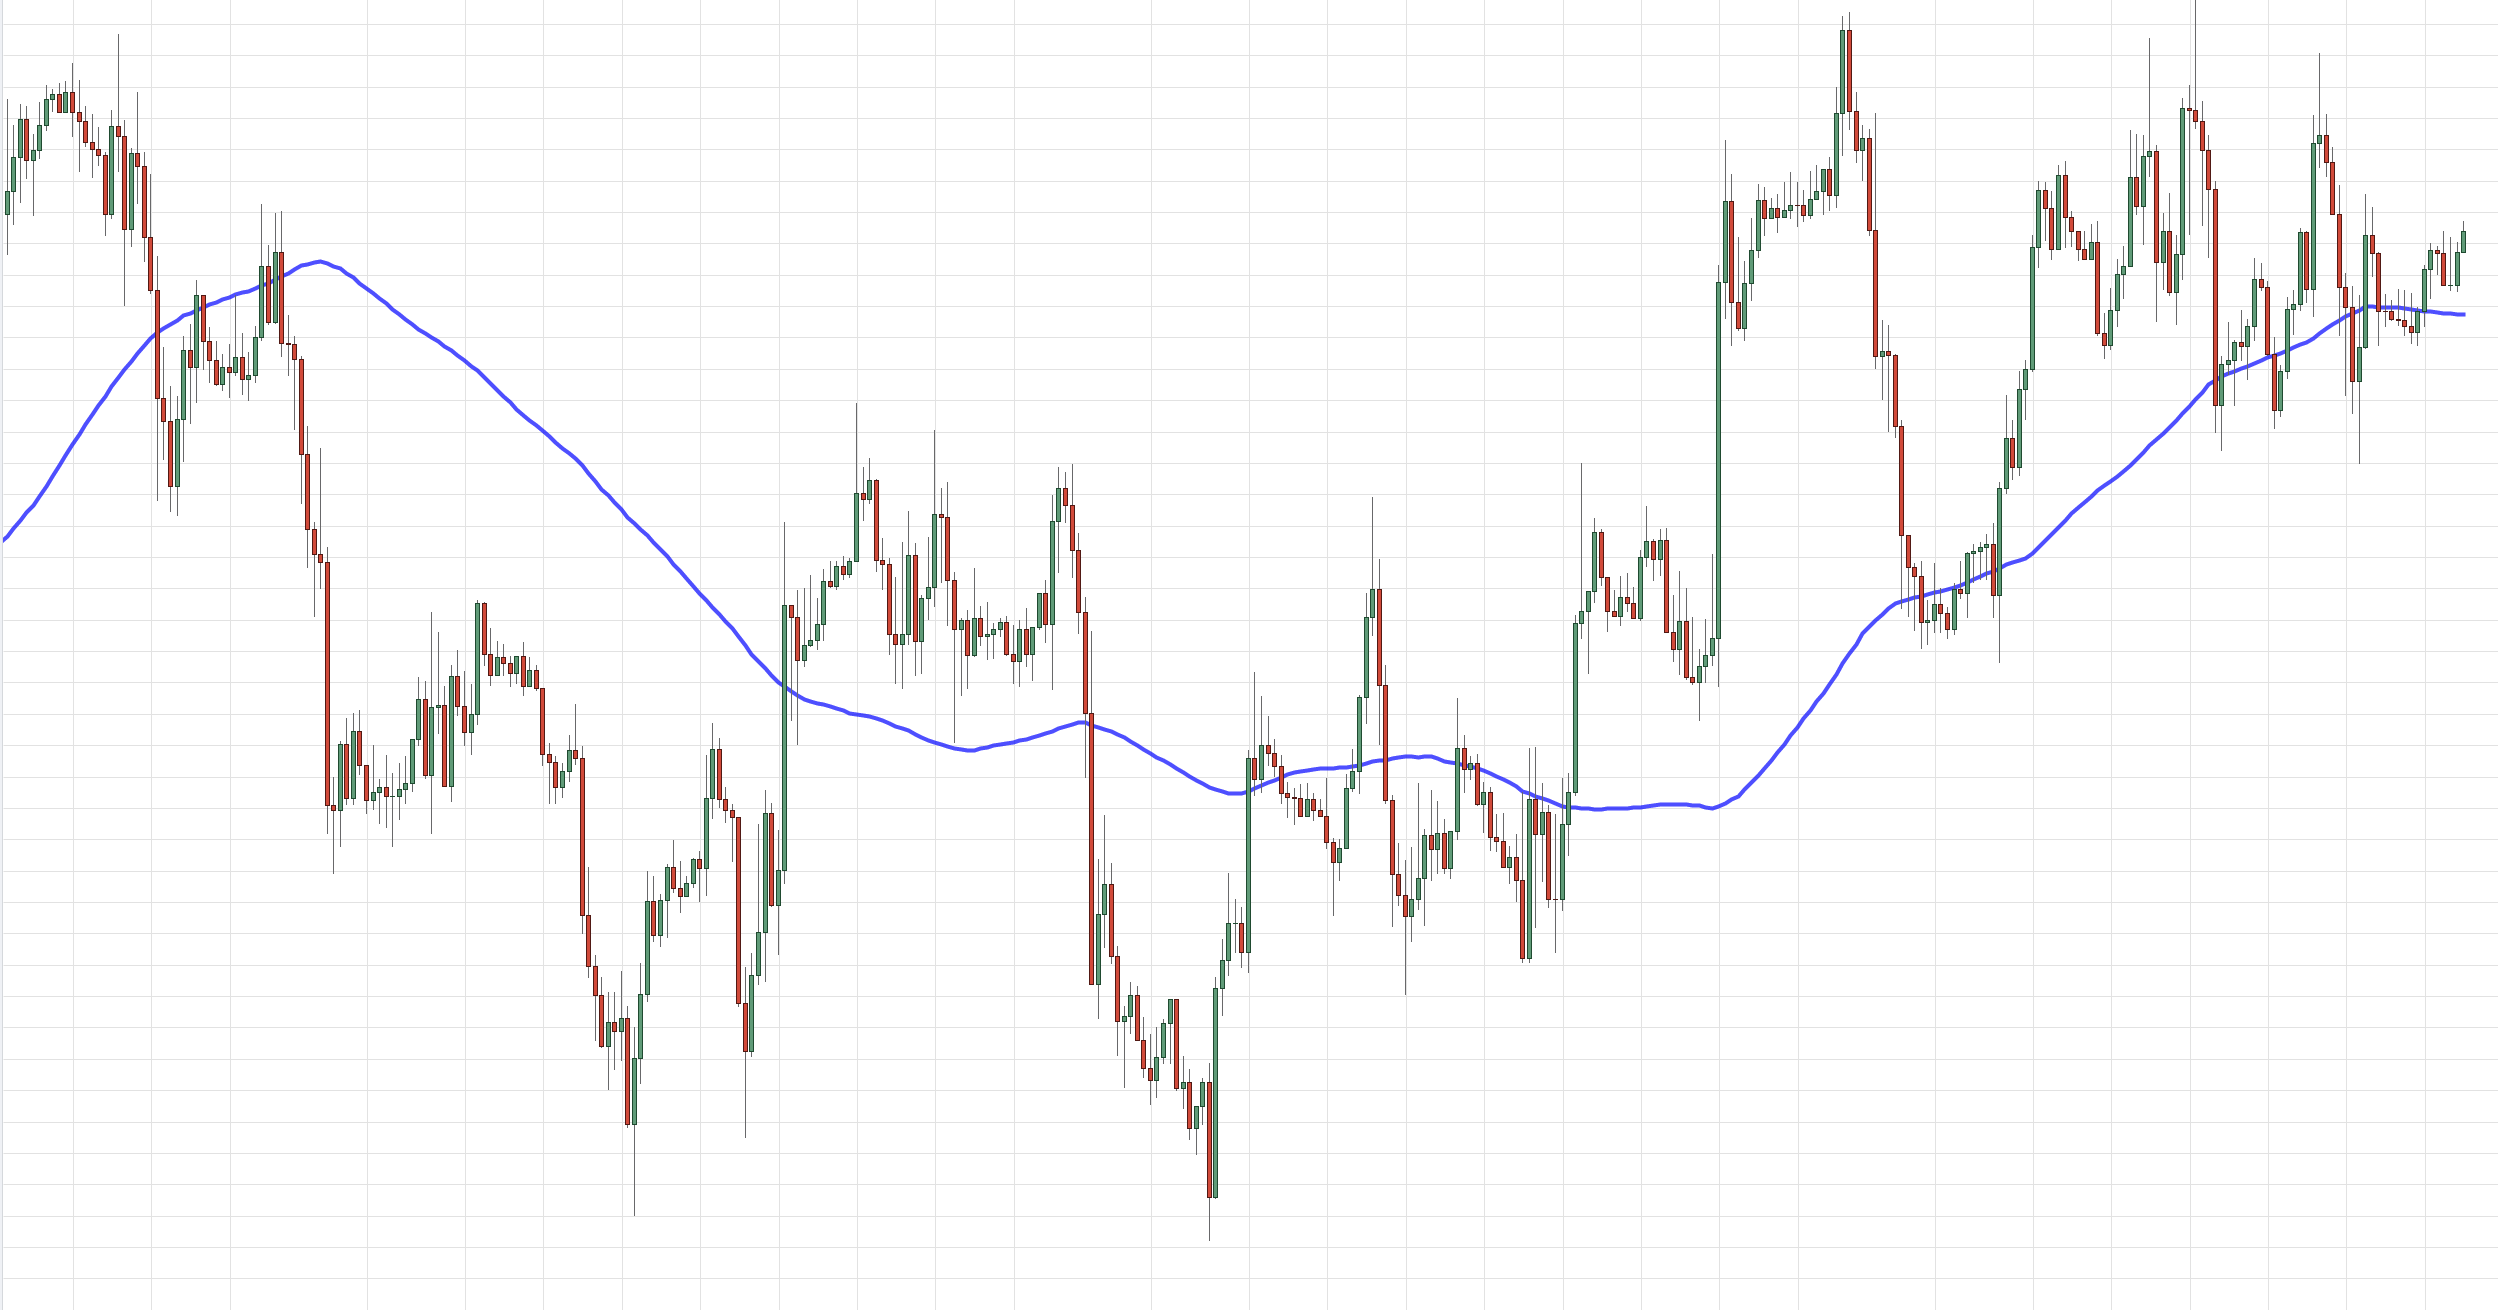
\includegraphics[width=0.8\textwidth]{img/fitting1.png}
% \label{figure:fitting1}
% \end{figure}

% \begin{figure}
% \caption{Fitting2}
% \centering
% 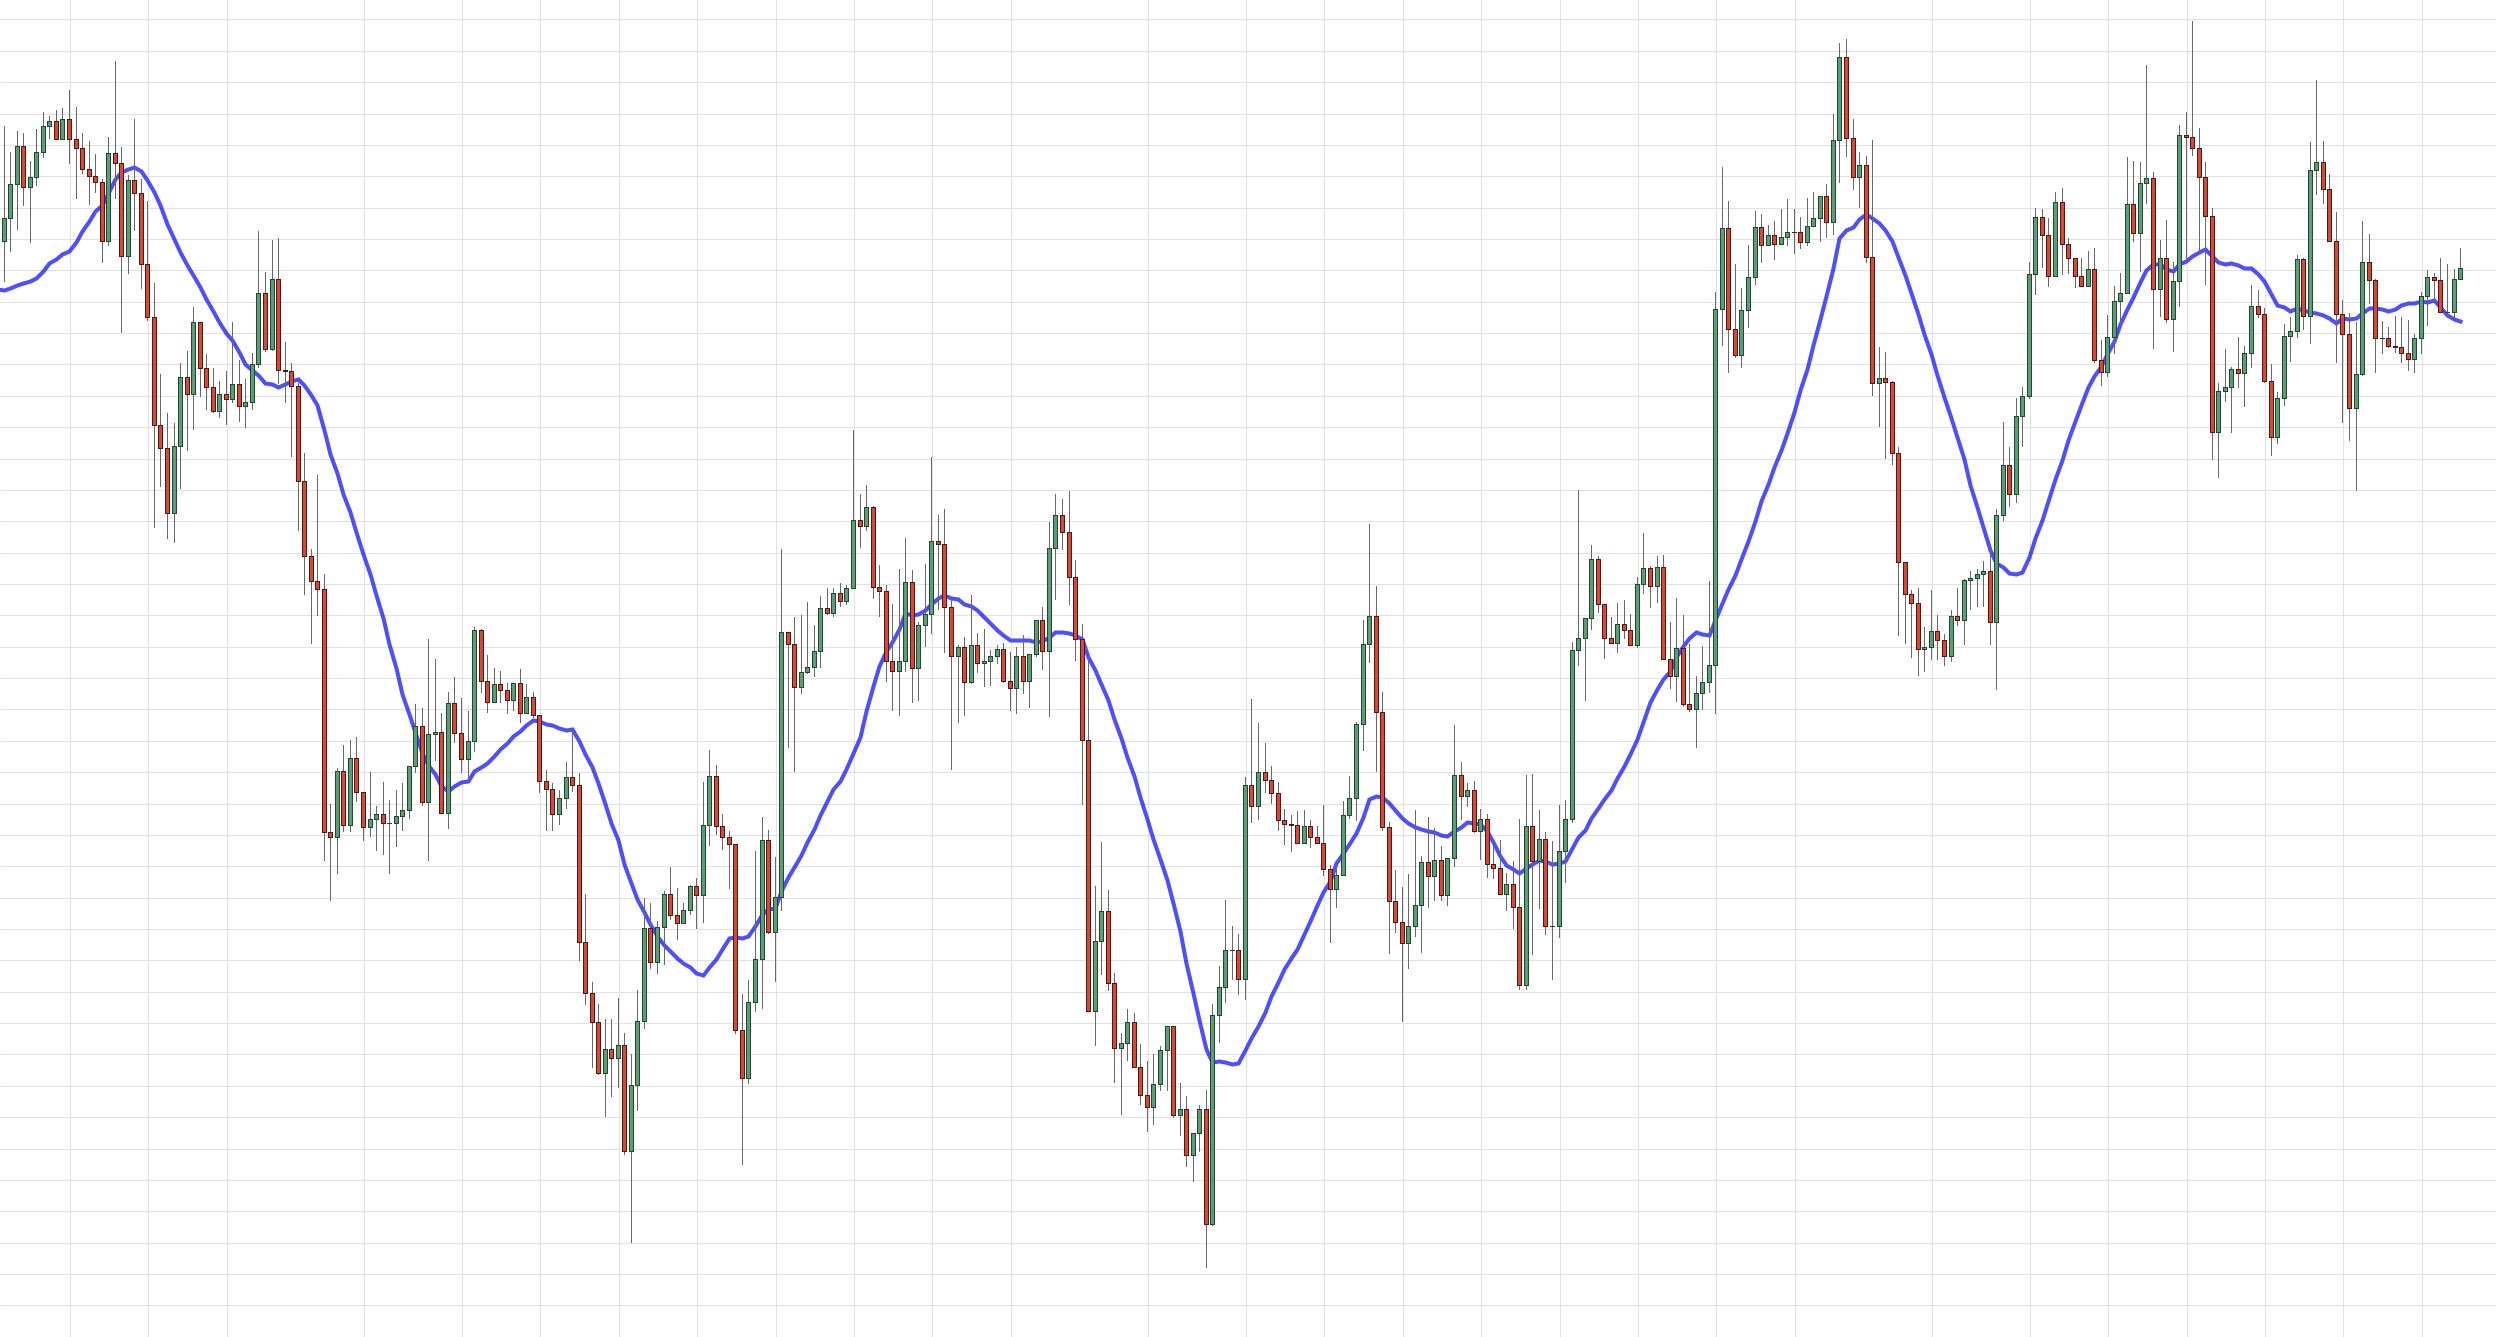
\includegraphics[width=0.8\textwidth]{img/fitting2.png}
% \label{figure:fitting2}
% \end{figure}

\section{Implementation}
\label{section:implementation}

\section{Experiments}
\label{section:experiments}

\subsection{Data Preprocessing}
\label{subsection:data-preprocessing}

Although the 

%% Talk about outputs using deltas. Inputs are prices (high, low, close).

\section{Results}
\label{section:results}

\section{Conclusion}
\label{section:conclusion}

\section{Future Work}
\label{section:future-work}

\section*{Acknowledgment}

\begin{IEEEbiography}[{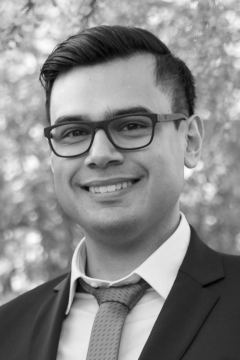
\includegraphics[width=1in,height=1.25in,clip,keepaspectratio]{img/amaury-1by1half-in.png}}]{Amaury
  Hernandez-Aguila} 
\end{IEEEbiography}

\bibliography{bibliography}
\bibliographystyle{IEEEtran}

\EOD

\end{document}
